\documentclass[a4paper,12pt,headsepline]{scrartcl}
\usepackage{amssymb}
\setcounter{tocdepth}{3}
%\setcounter{secnumdepth}{-2}
\usepackage{graphicx}
\usepackage{rotating}
\usepackage{float}
\usepackage{url}
\usepackage{hyperref}
\usepackage[ngerman,nameinlink]{cleveref}
\usepackage{array}
\usepackage{longtable}
\usepackage{listings}
\usepackage{color}
\usepackage{transparent}
\graphicspath{{Images/}}
\usepackage[utf8]{inputenc}
\usepackage{setspace}
\usepackage[ngerman]{babel}
\usepackage{fancyhdr}

\pagestyle{fancy}
\lhead{\leftmark}
\chead{}
\rhead{\rightmark}
\lfoot{}
\cfoot{\thepage}
\rfoot{}


\begin{document}
	\thispagestyle{empty}
	
	\begin{verbatim}
	
	
	\end{verbatim}
	
	\begin{center}
		\begin{figure} [H]
			\centering
			
\includegraphics[height=2cm]{Images/Logo_Uni-Kassel.png}
		\end{figure}
		\Large{Fachbereich 16 - Informatik und Elektrotechnik}\\
	\end{center}
	
	
	\begin{verbatim}
	
	
	
	
	\end{verbatim}
	\begin{center}
		\doublespacing
		\textbf{\LARGE{Teamarbeit}}\\
		\singlespacing
		\begin{verbatim}
		
		\end{verbatim}
		\textbf{Abschlussbericht}
	\end{center}
	\begin{verbatim}
	
	\end{verbatim}
	\begin{center}
		
	\end{center}
	\begin{verbatim}
	
	\end{verbatim}
	\begin{center}
		
	\end{center}
	\begin{verbatim}
	
	
	
	
	\end{verbatim}
	\begin{flushleft}
		\begin{tabular}{llll}
			\textbf{Autoren:} & & Dennis Knitterscheidt & 33360131 \\
			& & Robert Meschkat & 28227496\\
			& & Philipp Schenk & 33309370\\
			& & Eric Wagner & 32233447\\ \\
			\textbf{Betreuer:} & & M. Sc. Stephan Opfer &\\
		\end{tabular}
	\end{flushleft}
	\newpage
	\thispagestyle{empty}
	\tableofcontents
	\newpage
	
	\section{Einleitung}
Mit diesem Bericht werden der Verlauf und die Ergebnisse des Projekts, das im Rahmen der Veranstaltung Teamarbeit des Fachgebiets Verteilte Systeme entstand, dokumentiert. Im Verlauf von diesem Projekt sollten die Methoden und Techniken der Teamarbeit, die im Kickoff-Workshop erläutert wurden, genutzt werden, um die Erweiterung der Turtlebots um die Funktion als Transportsystem, mit dessen Hilfe verschiedene Dinge von Punkt zu Punkt gebracht werden können, zu implementieren.	
	\newpage
	\section{Technische Arbeit}
	
	\subsection{Arbeitsauftrag}
		Im Kickoff-Workshop zur Veranstaltung \glqq Teamarbeit\grqq\ hat sich das Team zusammen gefunden, um die folgende Aufgabe zu bearbeiten: \\
		Für die vom Team bearbeitete Aufgabe sollten ein Turtlebot und die existierende Software so erweitert werden, dass der Turtlebot als Transportsystem im Fachgebiet eingesetzt werden kann. Der Turtlebot sollte über die Software an einen Ort im Fachgebiet geschickt werden können, an dem er einen Gegenstand entgegen nimmt. Der Gegenstand sollte dann an einen vorher in der Software definierten Zielort gebracht werden. \\
		Für die Umsetzung sollte ein Behältnis  für den Transport der Gegenstände auf dem Turtlebot befestigt werden. Der Behälter sollte mit entsprechender Sensorik ausgestattet werden, damit der Turtlebot erkennt, wenn ein Gegenstand auf ihm platziert wurde. Da der Turtlebot nur Daten verarbeiten kann, die sich in seinem Weltmodell befinden, mussten die Sensordaten außerdem in das bestehende Framework eingepflegt werden.\\
		Um dem Turtlebot den Transportauftrag zu erteilen, sollte eine graphische Benutzeroberfläche entwickelt werden, in der man den Start- und Zielpunkt, sowie den zu transportierenden Gegenstand festlegen können soll.  

		
%		\begin{itemize}
%			\item Erstellen eines Transporters aus einem Turtlebot
%			\item Anbindung eines Drucksensors unter einen Tragekorb
%			\item Integration der Sensorwerte in das bestehende Framework
%			\item UI zum Steuern entwickeln
%			\item Testen und Evaluieren
%		\end{itemize}
	
	\subsection{Entwurf}
	\subsubsection{Erste Bestandsaufnahme}
		Da kein Teammitglied zuvor mit den Turtlebots gearbeitet hat, musste sich das Team zunächst einen groben Überblick über die bestehende Hard- und Software verschaffen, bevor mit der eigentlichen Planung begonnen werden konnte.\\
		Für die Sensorik des Behälters war der Aufbau des Turtlebots ausschlaggebend: Gesteuert wird der Turtlebot von einem Notebook. Dieses ist über USB sowohl mit der Fahrbasis, als auch mit der Sensorik für die räumliche Erkennung verbunden. Damit wurde klar, dass auch der Gegenstandsdetektor über USB mit dem Notebook verbunden werden musste. \\
		Die Software-Sammlung, die für den Betrieb des Turtlebots benötigt wird, basiert auf dem \glqq Robot Operating System\grqq , kurz ROS genannt, in der Version \textit{Kinetic}, und ist in C++ verfasst. Das User Interface musste also mit ROS kommunizieren können und im besten Fall in C++ geschrieben sein.

	\subsubsection{Recherche}
		Nachdem die Rahmenbedingungen abgeklärt waren, begann das Team zunächst mit der Suche nach Lösungen für die Aufgabenstellung.\\
		Bei der Sensorik für die Gegenstandserkennung hat sich das Team schnell auf einen Taster festgelegt, der ausgelöst werden soll, wenn ein Objekt in den Behälter gelegt wird. Kurzzeitig war auch noch ein RFID-Leser im Gespräch, der zusätzlich oder anstelle des Taster angebracht werden sollte. Mit dem Lesegerät hätten zwar die zu transportierenden Gegenstände identifiziert werden können, allerdings hätten dann auch alle Objekte mit einem entsprechenden Marker versehen werden müssen. Daher entschied sich das Team für den Taster, der beim Transport den größeren Spielraum lässt und außerdem leichter umzusetzen war. \\
		Für die mögliche Umsetzung des Tasters gab es verschiedene Lösungsansätze: Die einfachste Lösung wäre ein bereits fertiger Taster mit USB-Anschluss, der zum Beispiel eine Tastaturtaste simuliert. Die Recherche des Teams zeigte, dass entsprechende \glqq Ein-Knopf-Tastaturen\grqq\ tatsächlich existieren, sich jedoch preislich in keinem realistischem Rahmen bewegen. Ein weiterer Vorschlag war die Modifikation eines Peripheriegerätes, wie einer Maus oder einer Tastatur. Auch diese Idee wurde verworfen, da sie vom Team als zu aufwändig und als mögliche Fehlerquelle angesehen wurde. \\
		Für die Entwicklung des User Interfaces wurden zwei C++-Bibliotheken evaluiert: Zum einen der Quasi-Standard \glqq Qt\grqq\ und zum anderen das \glqq Chromium Embedded Framework\grqq , kurz CEF. Bei der Evaluation stellte sich das CEF als interessante Lösung heraus, wurde aber vom Team aber abgelehnt, da es für dieses Projekt als zu aufwändig eingeschätzt wurde.\\
		Als Plattform für die Entwicklung wollte das Team sowohl das im Fachgebiet eingesetzte Ubuntu 16.04 LTS mit ROS Kinetic, als auch das zu diesem Zeitpunkt aktuelle Ubuntu 18.04 LTS mit ROS Melodic erproben.

	\subsubsection{Erster Entwurf}	
		Nach der Recherche entschied sich das Team dazu, den Taster selbst zu bauen. Dafür sollte dieser mit einem Microcontroller verbunden werden, der die Signale über USB an das Notebook überträgt. Als Microcontroller wurde der \glqq Digispark Rev. 3\grqq\ (\cref{fig:digispark}) gewählt, da er mit seinen kleinen Abmessungen und seinem geringen Preis eine gute Lösung zu sein schien. 

		\begin{figure}[H]
			\centering
			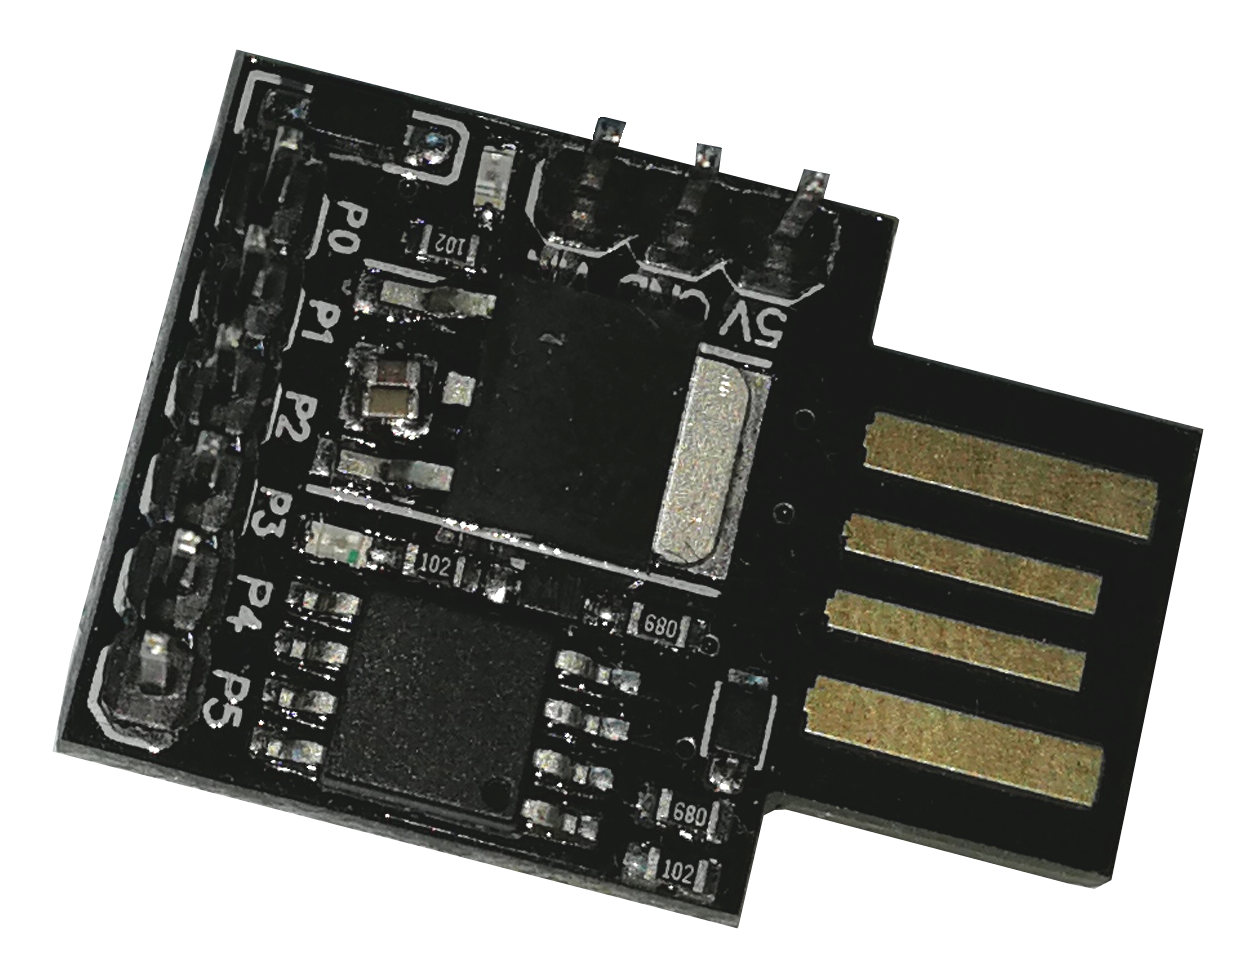
\includegraphics[width=4cm]{Images/digispark.png}
			\caption{Digispark Rev. 3}
			\label{fig:digispark}
		\end{figure}

		Für die Software untersuchte das Team den existierenden Code in den verschiedenen Git-Repositories und entwickelte aus den Ergebnissen einen ersten Ansatz für die Software-Architektur (\cref{fig:arch01}) des Projekts. Für den Client sollte dabei ein Frontend auf Basis von Qt entwickelt werden. Das Frontend schickt die Benutzereingaben an das Backend, welches die Daten verarbeitet und an ROS (bzw. die ROS-Kernanwendung) weiter reicht. Der existierende ROS-UDP-Proxy soll die Daten als ROS-Message über das WLAN an den Turtlebot schicken. Auf dem Turtlebot soll es eine ROS-Komponente geben, die die Daten in Kommandos für den Turtlebot umwandelt. 
		\begin{figure}[H]
			\centering
			\resizebox{\textwidth}{!}{\input{Images/architecture01.pdf_tex}}
			\caption{Erster Architektur-Entwurf}
			\label{fig:arch01}
		\end{figure}

	\subsubsection{Zweiter Entwurf} \label{sec:entwurf2}

		Nach Rücksprache mit dem Betreuer des Teams, Stephan Opfer, zeigte sich, dass die Software auf dem Turtlebot komplexer war, als zunächst angenommen: Wie in \cref{fig:arch02} zu erkennen ist, gibt es neben dem UDP-Proxy, Sensoren und Aktoren, auch noch ein Weltmodell und eine Komponente namens \glqq Alica\grqq . Im Weltmodell wird der von den Sensoren erfasste Zustand, sowie weitere Informationen, festgehalten. Alica kann sich den aktuellen Zustand aus dem Weltmodell holen, auf der Basis entsprechender Pläne das weitere Vorgehen ermitteln und das neue Verhalten an die Aktoren mitteilen. Für die Software auf dem Turtlebot musste das Team also keine eigene Komponente entwickeln, sondern den Taster in die Sensorik, das Weltmodell und die Pläne einpflegen, Außerdem musste eine Nachricht des Clients mit Start-, Endpunkt und Gegenstand ebenfalls in das Weltmodell eingetragen werden, damit diese Informationen ebenfalls in die Planung mit einbezogen werden können. \\
		Auf der Client-Seite erhielt das Team zusätzlich den Hinweis, dass es eine spezielle Version von Qt gibt, die direkt mit ROS kommunizieren kann, sodass die Aufteilung in Frontend und Backend nicht nötig ist.
		\begin{figure}[H]
			\centering
			\resizebox{\textwidth}{!}{\input{Images/architecture02.pdf_tex}}
			\caption{Zweiter Architektur-Entwurf}
			\label{fig:arch02}
		\end{figure}
%	\begin{itemize}
%		\item Turtlebot beschreiben
%		\begin{itemize}
%			\item Was ist der Turtlebot?
%			\item Was kann er?
%			\item Was wurde im Fachgebiet schon damit gemacht?
%		\end{itemize}
%		\item Verwendete Soft- und Hardware
%		\begin{itemize}
%			\item Grafik vom 14.05. einbauen und beschreiben 
%			\item Entscheidung für QT und RQT für die UI (Beschreiben)
%			\item Roboterprogrammierung in C++
%			\item Verwenden von QT oder Chromium für das Interface
%			\item Verwenden von Arduino mit Taster als Sensor
%			\item Optionale Idee: RFID-Leser mit Tags in Tassen oder Büchern
%		\end{itemize}
%	\end{itemize}
		
		
	\subsection{Umsetzung}
		Nach dem Kickoff-Workshop wurde vom Team beschlossen, sich einmal pro Woche im Labor des Fachgebiets zu treffen. Zu Beginn hat sich jedes Teammitglied mit Ubuntu und ROS beschäftigt und dieses auf seinem Rechnern installiert. Als Betriebssystem wurde Ubuntu 16.04 verwendet, da die Turtlebots mit ROS Kinetic arbeiten. Da der Turtlebot-Code aus mehreren GitHub-Repositories besteht, mussten diese zusätzlich heruntergeladen werden.\\
		Zuerst wurde in den Treffen mit einem Laptop mit Ubuntu-Version 18.04 versucht, den Code der Repositories zu kompilieren und auszuführen. Hierbei stieß man auf das Problem, dass einige Bibliotheken fehlten oder Code zum Teil nicht mit der neuen ROS-Version Melodic kompatibel war. Aufgrund dieses Problems wurde nach mehreren Kompilierungsversuchen auf einen Rechner im Labor des Fachgebietes umgeschwenkt, auf dem gemeinsam weiter programmiert wurde. Da auf dem Rechner trotz der korrekten Ubuntu-Version immer noch Dateien fehlten, wurde der Betreuer zu Rate gezogen. Neben einer Konkretisierung des Arbeitsauftrages (siehe \cref{sec:entwurf2}) stellte sich heraus, dass die verschiedenen Repositories unterschiedliche Branches benötigen, um richtig zu funktionieren und zusammenzuarbeiten. Dieses Problem betraf nicht den Laptop, der mit dem Turtlebot verbunden war, weswegen der Roboter bereits mit Hilfe eines rviz-Plugins fahren konnte.\\
		Nachdem die Repositories auf die korrekten Branches umgestellt wurden, konnte der Code kompiliert werden und das Team ließ den Turtlebot mit Hilfe des rviz-Plugins vom Rechner aus über den UDP-Proxy fahren. Während und nach der Arbeit an dem Problem des nicht kompilierenden Codes wurde gleichzeitig an dem Interface auf dem Rechner und dem Taster für den Turtlebot gearbeitet.
%		\begin{itemize}
%			\item Am Anfang Beschäftigung mit den Themen und Einarbeitung (Installation von Ubuntu und ROS)
%			\item Besprechung mit dem Betreuer zu Konkretisierung des Auftrags
%
%			\item Probleme durch Betriebssystem und Branches erwähnen
%			\item Verwendung von Linux 16.04 als Betriebssystem
%			\item Parallele Arbeit an Taster und UI
%			\item Nachdem Laptop nicht funktioniert hat wurde auf den Rechner umgeschwenkt
%		\end{itemize}

	\subsubsection{UI}
		Das User Interface (UI) wurde mit Hilfe der Software QtCreator in Qt erstellt. Im QtCreator kann der Nutzer leicht Bedienelemente in einen Fensterdesigner hineinziehen. Das fertig designte Fenster kann als \glqq .ui\grqq-Datei gespeichert werden. Für diese UI-Datei wurde danach in C++ eine Header- und Implementations-Datei mit den Namen \glqq rqt{\_}turtlebutler\grqq\ geschrieben.\\
		Das Interface wurde zuerst von Eric zu Hause erstellt und danach gemeinsam in den Team-Treffen fertig gestellt. Die erste Version der UI enthielt noch Fehler im Programmcode. Diese wurden zusammen behoben und die UI konnte zum ersten Mal am 9. Juli kompiliert werden.
		\begin{figure} [H]
			\centering
			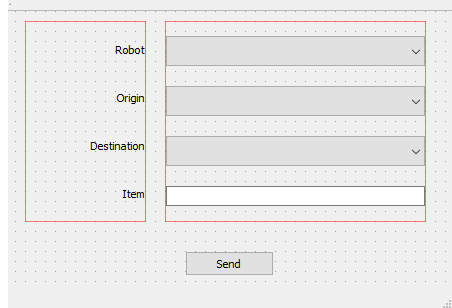
\includegraphics[height=6cm]{Images/Turtlebutler_Old.png}
			\caption{Alte Version des User-Interfaces in QtCreator}
			\label{fig:OldUI}
		\end{figure}
		Wie auf \cref{fig:OldUI} zu erkennen ist, bestand die erste Version der UI aus einer Reihe an Dropdown-Menüs mit einem Knopf. Im ersten Dropdown-Menü konnte der Nutzer zwischen einem der drei Roboter des Fachgebiets, Leonardo, Donatello und Raphael, wählen. Die nächsten zwei Menüs dienten zur Auswahl des Abhol- und Zielpunktes. Zuletzt konnte mit einer Texteingabe der gewünschte Gegenstand angegeben werden. Durch das Drücken des Sendeknopfes sollten diese Informationen nun in einer Nachricht verpackt werden, die an den gewählten Turtlebot geschickt werden sollte.\\
		In der ersten Version wurde zunächst eine Konfigurationsdatei namens \glqq turtlebots.txt\grqq\ angelegt, die Informationen zu den Turtlebots und festgelegten Punkten auf der von einem Turtlebot aufgenommenen Karte des Fachgebiets enthielt. Die Daten in der Datei wurden mit Hilfe von Semikolons und Zeilenumbrüchen getrennt. Zuerst wurden hier die Roboternamen mit ihren ROS-Topics gelesen und danach die Standortnamen mit deren X- und Y-Koordinaten.  Die gelesenen Daten wurden danach in die jeweiligen Dropdown-Menüs geschrieben. Der Nutzer konnte dadurch die Namen von Turtlebots und Standorten sehen.\\
		Da die Nachrichten ohne ein passendes Planungs- oder Behaviour-Skript auf der Roboter-Seite nicht funktionierten, wurde zunächst eine simplere Nachricht verschickt. Hierfür wurde aus dem existierenden rviz-Plugin für den Turtlebot die jeweiligen ROS-Topics der Roboter und der Typ der Nachricht entnommen. Es handelt sich dabei um eine \glqq Posed\_Stamped\grqq -Nachricht, die die Koordinaten des gewählten Zielpunkts enthält. Erhält der Turtlebot mit den bereits existierenden Plänen die Nachricht, so fährt er zu der gegebenen Position auf der Karte.\\
		Beim Erstellen der Konfigurationsdatei hat sich herausgestellt, dass für jede Position in der Datei von Hand eine Nachricht mit dem rviz-Plugin verschickt und deren Position notiert werden muss. Aufgrund dessen wurde nach einem Gespräch mit dem Betreuer entschieden, die bereits existierende Datei namens \glqq TopologicalModel.conf\grqq\ zu verwenden. In dieser befindet sich eine Sammlung von \glqq Points of Interest\grqq\ (POIs) der Räume des Fachgebiets basierend auf einer optimierten Karte.\\
Zum Einlesen der Datei konnte auf das existierende Paket \glqq SystemConfig\grqq\ zurückgegriffen werden. Es liest die Datei ein und stellt die Daten geordnet über entsprende Methoden zur Verfügung. Die eingelesenen Daten konnten dann in eine Map gespeichert werden, die jedem Raum eine Liste von Points of Interests zuordnet.\\


		\begin{figure} [H]
			\centering
			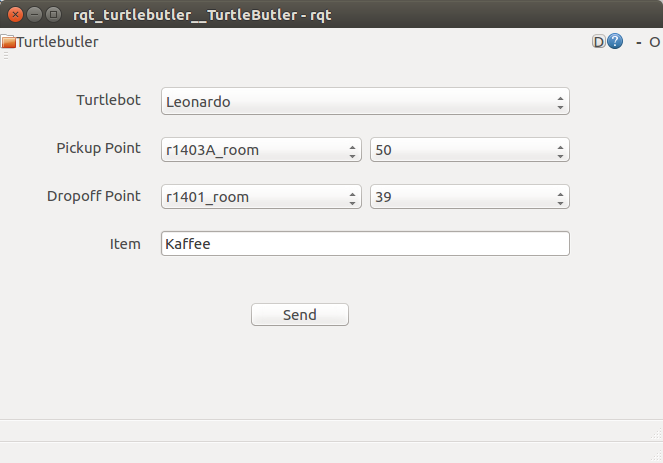
\includegraphics[height=8cm]{Images/Turtlebutler_Used.png}
			\caption{Aktuelle Version des User-Interfaces}
			\label{fig:NewUI}
		\end{figure}
		Aufgrund der neuen Datenstruktur der POIs musste auch die UI verändert werden. Wie man an \cref{fig:NewUI} und \cref{fig:NewUIDropdown} sehen kann wurden die Dropdown-Menüs der Positionen in zwei Teile aufgeteilt. In dem linken Menü kann der Nutzer den Raum bestimmen und in dem rechten die Position im Raum. Wählt der Nutzer einen Raum, so ändert sich dadurch die Liste an verfügbaren Positionen. Für das Verschicken der Nachricht ist hierbei nur die Position relevant, da diese mit den X- und Y-Koordinaten verknüpft ist, die der Turtlebot benötigt. Da das Behaviour-Skript leider nicht fertig gestellt werden konnte, verschickt die neue UI weiterhin nur die Abholposition als \glqq Pose{\_}Stamped\grqq-Nachricht.
		\begin{figure} [H]
			\centering
			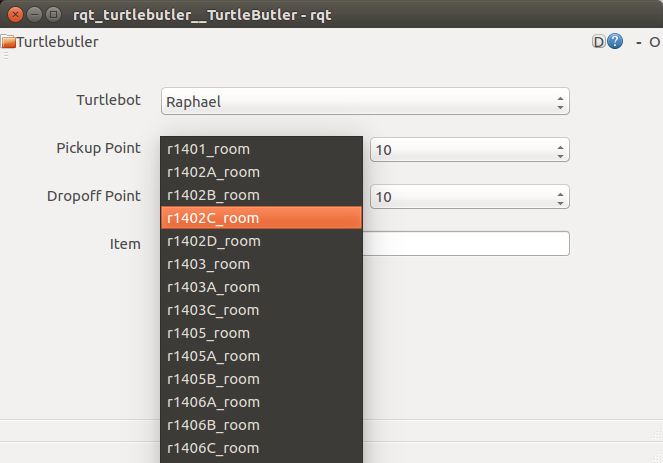
\includegraphics[height=5cm]{Images/Turtlebutler_Rooms.png}
			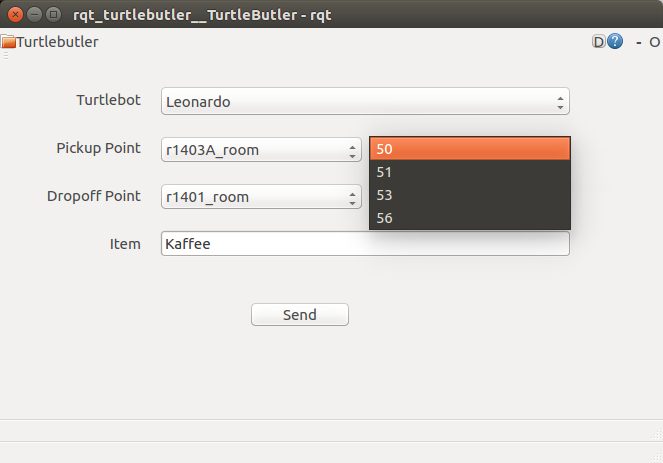
\includegraphics[height=5cm]{Images/Turtlebutler_Positions.png}
			\caption{Dropdown-Menüs des neuen User-Interfaces}
			\label{fig:NewUIDropdown}
		\end{figure}
	
%		\begin{itemize}
%			\item Verwenden von QTCreator zum Erstellen des UI-Fensters
%			\item Schreiben des Codes mit C++ und ROS (RQT)
%			\item Erstellen der UI zu Hause
%			\item Bugfixen auf dem Rechner als Team
%			\item Nachrichtenart vom rviz Plugin entnommen (Pose{\_}Stamped)
%			\item Erste Version zeigen (Bild) und beschreiben
%			\item Erste Version der Datenstruktur beschreiben
%			\item Fehler in der UI-Entwicklung beschreiben und Verbesserungen sagen
%			\item Error Handling bei schlechter Config Datei
%			\item Umstellung auf existierende Kartendaten mit anderer Struktur (Karte entspricht nicht der Roboterkarte) (Robert)
%			\item Verbesserung der UI mit den neuen Punkten (Zweite Version zeigen)
%		\end{itemize}
			
	\subsubsection{Taster}
\begin{figure} [H]
\centering
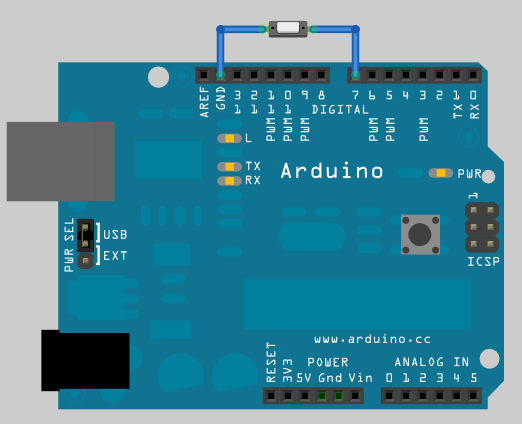
\includegraphics[height=5cm]{Images/button_hardware.png}
\caption{Skizze des Arduino-Boards}
\label{fig:arduinotaster}
\end{figure}
	
	Die Tastereingabe wurde durch einen zweipoligen Drucktaster und einen Arduino realisiert. Der Arduino wurde gewählt, da er das analoge Signal des Tasters entprellt, digitalisiert und in eine ROS-Message umwandelt. Ein Arduino Mega 2560 und ein Drucktaster waren bereits vorhanden und boten sich daher für die erste Realisierung an. Weil kein weiteres Material erforderlich war, stellte sich dies als die kostengünstigste und schnellste Methode für die Umsetzung der Tastereingabe heraus. Durch den eingebauten Pull-up-Widerstand im Arduino konnte der Taster direkt über zwei Leitungen mit dem Arduino verbunden werden, wie in \cref{fig:arduinotaster} zu sehen ist. Beim Öffnen des Tasters bekommt der Arduino ein HIGH-Signal. Da allerdings ein schließender Taster verwendet wird, musste dieser bei der Programmierung des Arduino invertiert werden. Die Umwandlung des Taster-Signals in die benötigte ROS-Message erfolgt über eine speziell dafür entwickelte Arduino/ROS-Kommunikationsbibliothek namens \glqq rosserial\_arduino\grqq, welche zusätzlich installiert werden musste. Beim Code für den Arduino wurde sich an einem Internet-Tutorial orientiert. Damit nicht kontinuierlich ROS-Messages versendet werden, wurde in das Arduino-Programm eine Verzögerung zwischen jeder abgesendeten Nachricht von einer Sekunde eingebaut. Zum Testen der Kommunikation wurde der Taster an den Arduino angeschlossen und in zufälligen Abständen betätigt. Wie erwartet war die ROS-Message im Linux-Terminal zu sehen.\\
Um den Taster in das Weltmodell des Turtlebots einzufügen, musste auf dem Turtlebot als erstes die passende Version von \glqq rosserial\grqq\ installiert werden, sodass man den dazugehörigen ROS-Node starten und diesem die serielle Schnittstelle des Arduinos übergeben kann. Mit diesen Vorbereitungen konnte der Arduino ROS-Nachrichten verschicken, mit denen der Turtlebot weiterarbeiten kann. Damit die Daten des Tasters auch vom Turtlebot registriert werden konnten, mussten als erstes in der Datei \glqq Communication.h\grqq\ ein Subscriber und eine Funktion, die bei einer empfangenen Nachricht ausgeführt wird, deklariert werden. In der Datei \glqq Communication.cpp\grqq\ wurde der Subscriber mit dem passenden Topic des Arduinos initialisiert, welches in der Konfigurationsdatei hinterlegt ist. Die Funktion wurde so implementiert, dass sie die Daten an den Programmteil weitergibt, der sich um die rohen Sensordaten kümmert. Die Sensordaten wurden von der neu deklarierten Funktion \glqq processTransportSystemState\grqq\ in der Datei \glqq RawSensorData.h\grqq\ weiterverarbeitet. Ebenfalls deklariert wurden hier ein Buffer samt Getter, in den die Funktion die Daten speichert, und die Zeitspanne der Validität der Daten. Die Implementierung von \glqq processTransportSystemState\grqq\ erfolgte in der \glqq RawSensorData.cpp\grqq. Dort wurden auch der Buffer und die Zeitspanne der Validität mit den entsprechenden Konfigurationsdaten initialisiert. Die Konfigurationsdaten für die Zeitspanne der Validität unserer Daten, das Topic und die gewollte Größe des Buffers mussten in der Datei \glqq TTBWorldModel.conf\grqq\ hinzugefügt werden.\\
\begin{figure}[h]
\begin{minipage}[t]{0.45\linewidth}
\centering
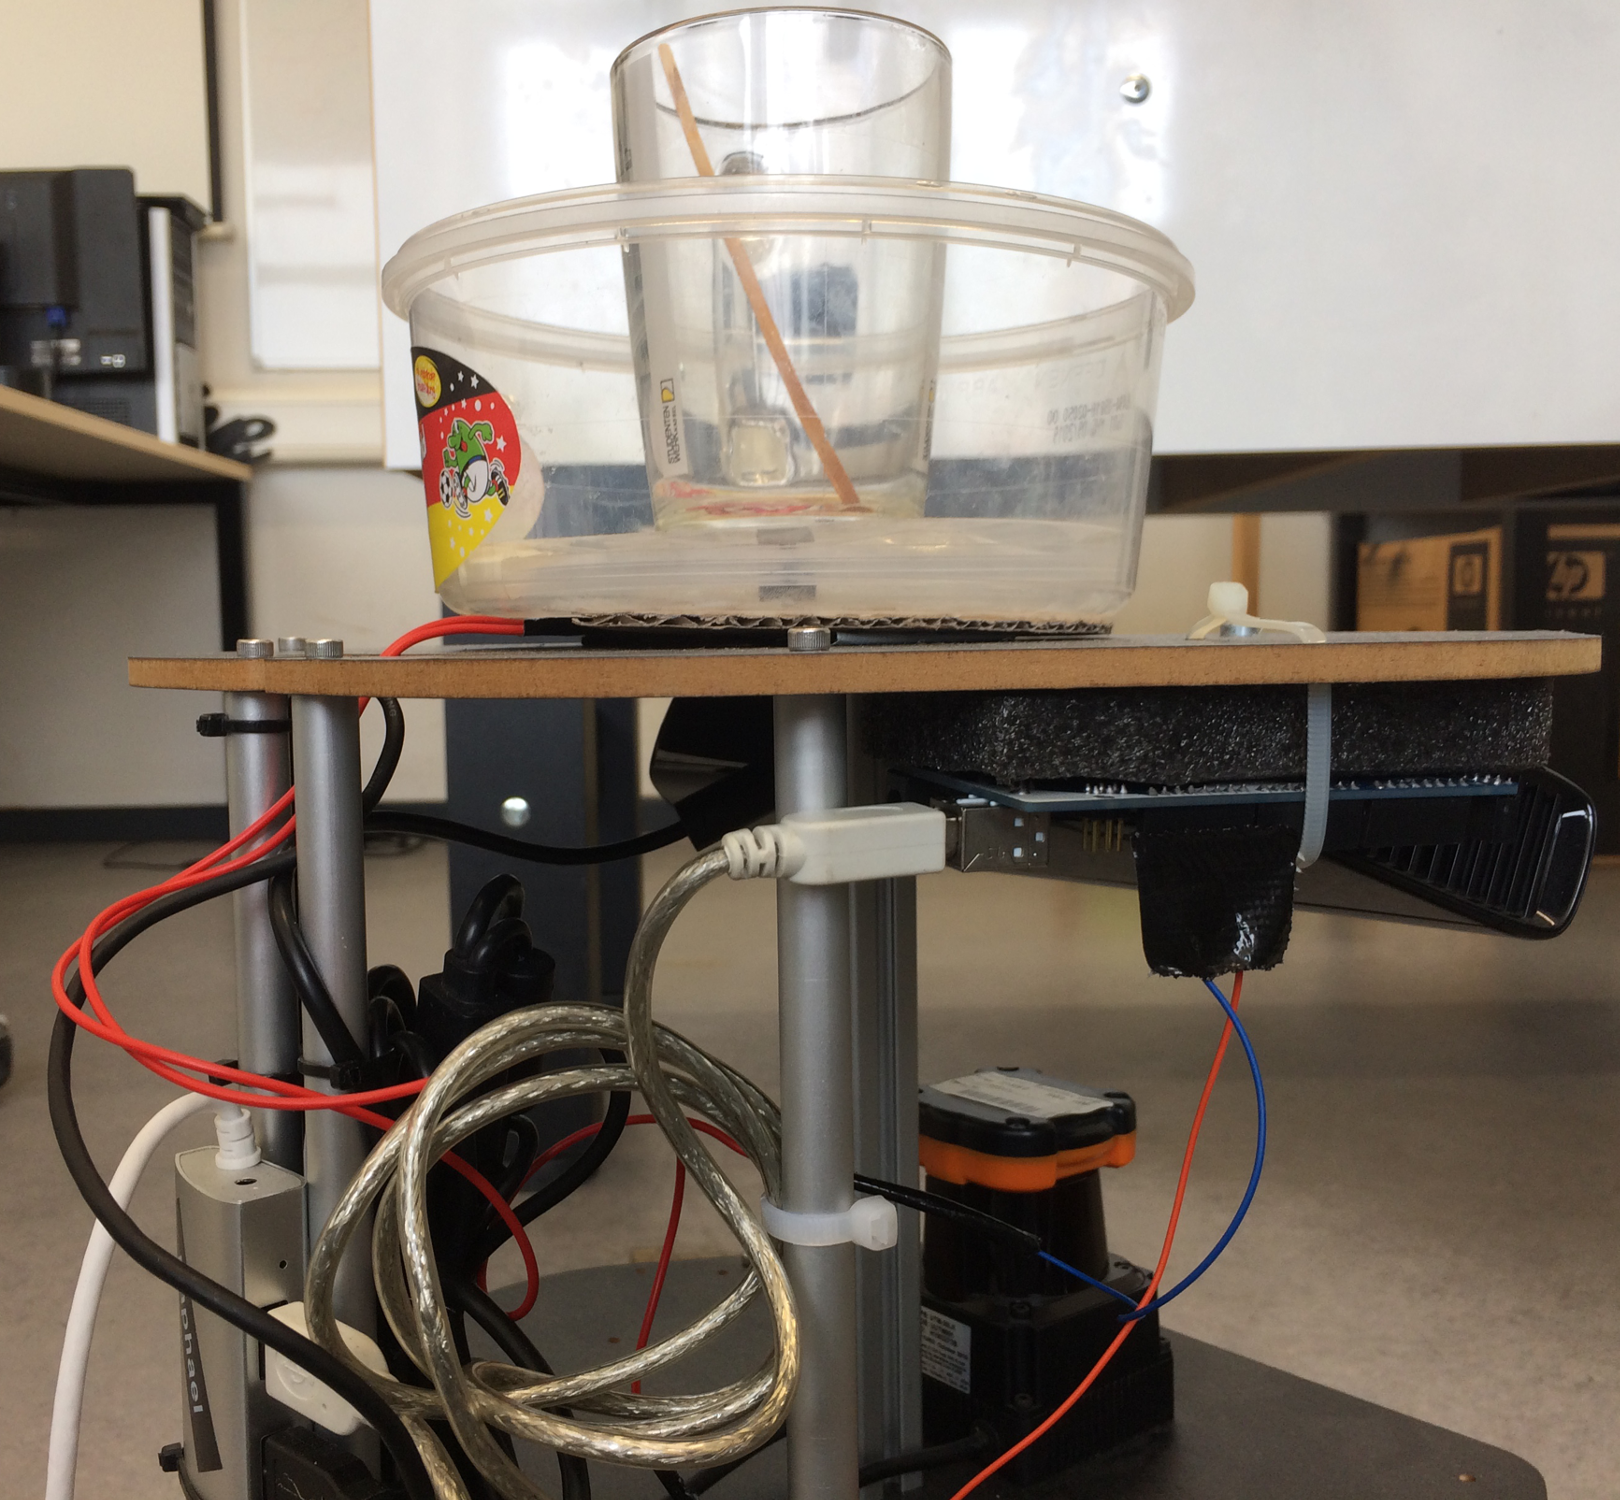
\includegraphics[height=5cm]{Images/Taster01.png}
\caption{Turtlebot mit Taster-Box}
\label{fig:taster01}
\end{minipage}
\hfill
\begin{minipage}[t]{0.45\linewidth}
\centering
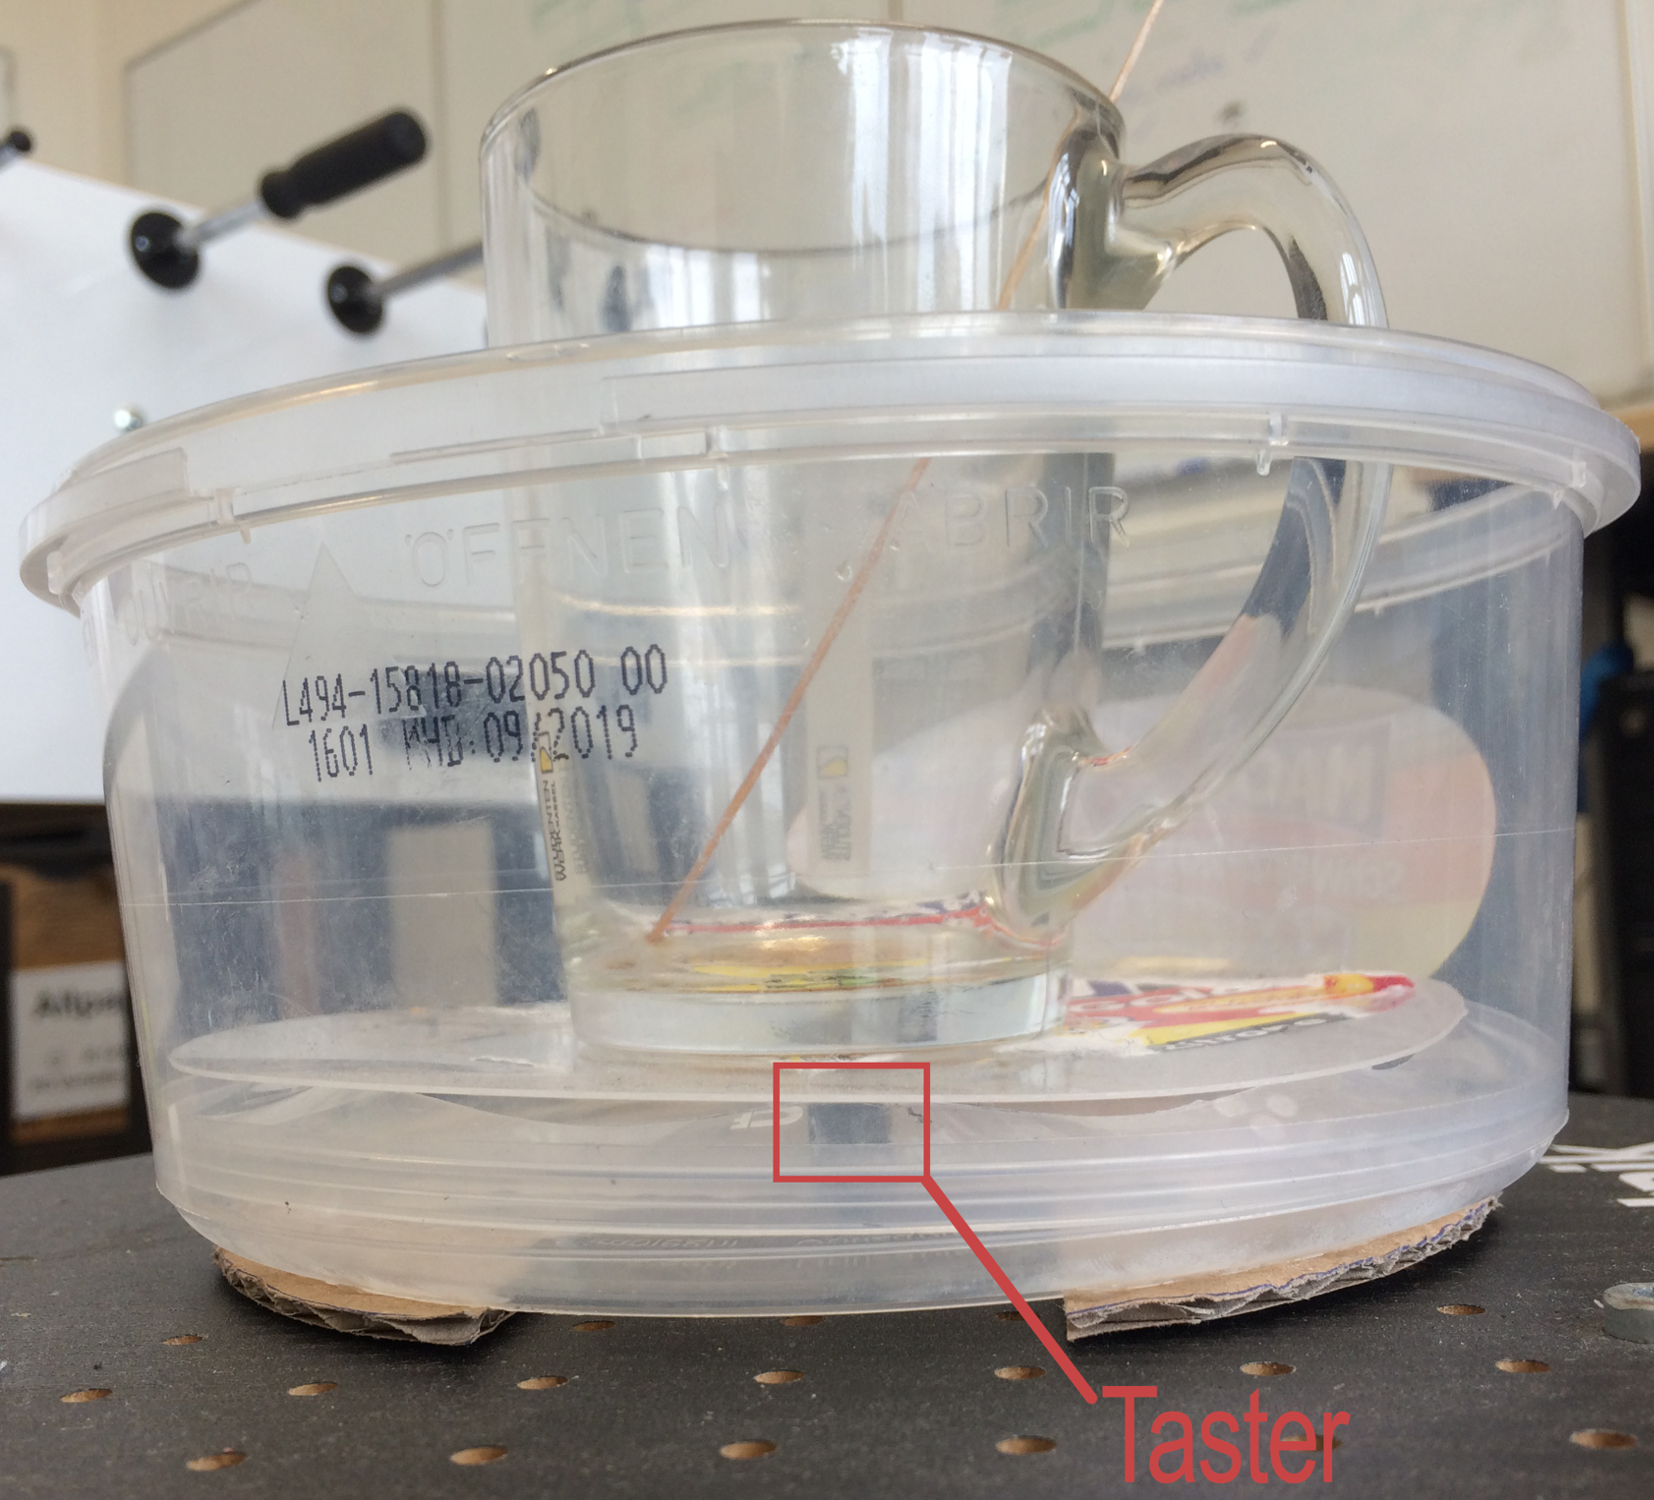
\includegraphics[height=5cm]{Images/Taster02.png}
\caption{Box mit erkennbarem Taster}
\label{fig:taster02}
\end{minipage}
\end{figure}

Im Kickoff-Workshop wurde besprochen, was der Roboter als Eingabequelle für den Taster entgegennehmen soll. Es wurde sich zum Schluss auf eine Kaffeetasse geeinigt, welche den Taster aktivieren soll. Handelsübliche Drucktaster sind in günstigen Ausführungen recht klein und nicht dafür geeignet, dass direkt ein Objekt in der Größe einer Tasse auf sie gestellt werden. Um dieses Problem zu beheben, musste eine Vorrichtung gebaut werden, welche ein definiertes Druckverhalten einer großen Fläche an den Drucktaster weitergibt. Der Betreuer des Teams empfahl, diese Vorrichtung aus einem Plastikkorb mit darunterliegendem Taster zu realisieren. Dies stellte sich aber als recht schwierig heraus, da die Böden solcher Plastikkörbe recht dick sind und das Gewicht einer Tasse meist nicht ausreicht, um den Taster zu aktivieren. Außerdem ist es schwierig, einen definierten Druck auf der gesamten Fläche des Korbes zu realisieren. Dennis hat zuhause versucht, diese beiden Probleme in den Griff zu bekommen und trotzdem kostengünstig zu bleiben. Als Lösung ist dabei eine große, verbaute Haribo-Box zustande gekommen, wie in \cref{fig:taster01} zu sehen ist. Der Taster ist ein THT-Drucktaster mit zwei langen Beinen. Diese wurde durch den Boden der Haribo-Box gestochen und mit etwas Kleber fixiert. Damit die Haribo-Box auf den Boden gestellt werden kann, musste noch eine Höhendifferenz aus Pappe unter den Boden geklebt werden, damit die Beinchen des Tasters nicht das darunter liegende Objekt berühren. Zwischen den beiden Pappstücken am Boden entstand dadurch ein dünner Kanal, in dem zwei Anschlussleitungen verlegt werden konnten, welche anschließend an die beiden Beinchen des Tasters gelötet wurden. Der Rand des Deckels wurde abgeschnitten und an beiden Enden überlappend an den inneren Boden der Box geklebt, um einen Abstand zu realisieren. Der Rest des Deckels, eine kreisrunde Scheibe, wurde anschließend in die Box auf den Taster gelegt. Durch den Rand am inneren Boden wird garantiert, dass die Scheibe nicht viel Spielraum hat und bei Belastung nicht den inneren Boden berührt. Getestet und genauer spezifiziert wurde die Box dann mit einem Digital-Multimeter und einer Haushaltswaage. Die beiden Anschlussleitungen wurden an dem Messgerät angeschlossen und das Messgerät auf Durchgang gestellt. Mehrere Objekte mit unterschiedlichem Gewicht zwischen 100g und 1kg wurden gewogen und anschließend in die Box auf unterschiedliche Stellen der Scheibe gestellt. Resultat des Versuchs war, dass die Box Gegenstände an allen Stellen auf der Scheibe ab einem Gewicht von etwa 200g erkennt. Eine normale Kaffeetasse ohne Inhalt wiegt etwa 300g. Damit sind die Anforderungen an die Box erfüllt. Der Arduino und die Taster-Box wurden dann beim Teamworktermin am 09.08.2018 am Turtlebot mit Kabelbindern und Schaumstoff befestigt und anschließend noch einmal kurz zur Demonstration getestet.
%\begin{itemize}
%\item Rosserial Arduino zur Umwandlung in Nachrichten
%\item Entscheidung für Arduino
%\item Schreiben des Codes und Bauen des Tasters
%\item Einbauen des Tasters in das Weltmodell (Philipp)
%\item Verbesserung des Tasters mit Korb aus Haribo
%\end{itemize}
	
	\subsection{Ausblick}
		Leider konnte der ursprüngliche Arbeitsauftrag aufgrund von technischen Komplikationen am Anfang und fehlender Zeit nicht zu Ende geführt werden. Das User Interface zum Verschicken der Nachrichten und der Taster zum Überprüfen von Gegenständen konnten zu einem Großteil fertiggestellt werden.\\
		Das Interface lädt im Moment Kartendaten einer idealen Karte, die nicht den Schlupf der Räder des Turtlebots mit einbeziehen. Dadurch kann es sein, dass der Roboter bei längeren Fahrten seine Position verliert oder nicht an seinem Ziel ankommt. Deswegen müssen die momentan verwendeten Points of Interest mit Hilfe von Roboter-Informationen angepasst werden. Neben den idealisierten Positionen schickt die UI nur für den Abholpunkt eine \glqq Pose{\_}Stamped\grqq-Nachricht. Diese sollte durch ein anderes Nachrichtenformat ersetzt werden, das beide Zielorte und den aufzunehmenden Gegenstand zusammen mit dem Absender enthält.\\
		Der Taster wurde bereits in das Weltmodell eingebaut und aktualisiert seinen Wert jede Sekunde. Diese Daten müssen noch in einem Behaviour verarbeitet werden. Das fehlende Planungsbehaviour soll die Nachricht mit dem neuen Format verarbeiten und den Turtlebot zuerst zu dem Abholpunkt fahren lassen. Wird der Taster gedrückt, so soll sich der Roboter kurz danach zu dem Zielpunkt bewegen. Ist ein Turtlebot unterwegs zu einem Abhol- oder Zielpunkt, so soll dieser nicht verfügbar sein, und dem Rechner eine entsprechende Antwort schicken.\\
		Während der Entwicklungszeit gab es zusätzliche Ideen, mit denen das Transportsystem erweitert werden kann. Zum einen könnte man auf dem Laptop ein Text-to-Speech-Programm verwenden, dass den in der Nachricht beschriebenen Gegenstand über die Lautsprecher ausgibt. Somit wüssten auch Unbeteiligte, was der Turtlebot abholen soll. Neben einer Sprachausgabe könnte man auch einen RFID-Leser in den Tragekorb einbauen, der beispielsweise auf RFID-Tags in Büchern oder Tassen reagiert. Dadurch kann der Turtlebot nicht nur überprüfen, dass etwas in dem Korb liegt, sondern auch welcher Gegenstand genau sich dort befindet.
		
%		\begin{itemize}
%			\item Auftrag ist nicht ganz fertig geworden
%			\item Schreiben eines Behaviours, das den Taster verwendet
%			\item Verwenden von anderen Nachrichtentypen zum Senden
%			\item Anpassen der Kartendaten mit Roboter-Infos
%			\item Roboter kann per Text to Speech den gesuchten Gegenstand sagen
%			\item Verwendung von RFID zur Erkennung der Gegenstände
%		\end{itemize}

	\newpage
	\section{Teamarbeit}
	
	\subsection{Teamrollen}
		In dem Kickoff-Workshop wurden zwei Aufteilungen von Teamrollen vorgestellt: Basadur und Belbin. In den folgenden Abschnitten haben sich die Teammitglieder gemeinsam in den verschiedenen Modellen eingeordnet.
	\subsubsection{Dennis}
Im Kickoff-Workshop hatte sich Dennis im Teamrollen-Modell von Basadur als eine Mischung aus \textbf{Conceptualizer} und \textbf{Implementer} eingeordnet, da er versucht, ein Problem zuerst oberflächlich aber vollständig zu begreifen und dann erste Lösungsansätze meist praktisch zu realisieren. Im Laufe der Zeit verschob sich seine Rolle als \textbf{Conceptualizer} eher zum \textbf{Optimizer}. Dadurch, dass das Projekt sehr programmierlastig war, hat Dennis versucht, die Ideen der anderen mit seinen Kenntnissen so gut es ging zu realisieren. Im Modell von Belbin sah sich Dennis als eine Mischung aus \textbf{Weichensteller} und \textbf{Umsetzer}, da er durch seine extrovertierte Art keine Hemmungen hat, mit Menschen innerhalb und außerhalb des Teams zu kommunizieren und weil er einen Sinn für das Praktische hat. Dies bestätigte sich im Laufe der Zeit. Außerdem übernahm er noch die Rolle als \textbf{Spezialist}, da er sich als einziger Elektrotechniker um den Hardware-Teil des Projekts kümmern konnte. Seine Rollen liegen in allen drei Orientierungsbereichen des Modells. Dadurch, dass das Projekt sehr programmierlastig war, fühlte sich Dennis zeitweise unbrauchbar für die Lösung mancher Probleme. Andererseits konnte er durch aufmerksames Zuschauen und Zwischenfragen auch das ein oder andere für die Zukunft dazulernen.
\subsubsection{Robert}
Im Kickoff-Workshop hatte sich Robert im Teamrollen-Modell von Basadur als \textbf{Conceptualizer} eingeordnet, da er für Probleme gerne erst einen Lösungsansatz entwickelt, bevor er diese angeht. Diese Einschätzung hat sich gerade zu Beginn des Projekts bestätigt, da er zum Beispiel die ersten Grafiken für eine mögliche Architektur entwickelt hat. Im Laufe des Projekts zeigte sich jedoch auch eine Tendenz zum \textbf{Implementer}, da nach Roberts Empfinden je nach Problem durch Ausprobieren und Testen schneller Erfolge erzielt wurden. Weniger sieht sich Robert als \textbf{Optimizer}. Ideen in Lösungen umzusetzen fällt ihm ohne weiteren Input schwer. Das trifft vor allem zu, wenn die Ideen oder Konzepte nicht von ihm selbst stammen.\\
Bei Belbin sah sich Robert vor dem Projekt hauptsächlich in der der Rolle des \textbf{Perfektionisten}, da er sich für nachhaltige Problemlösungen einsetzt und sich gerne auch mal in kleine Teilprobleme verbeißt. Auch diese Einordnung lässt sich nach dem Projekt bestätigen, da er zum Beispiel bei einigen Problemen auf sauberere Lösungen bestanden hat, die jedoch mehr Zeit in Anspruch genommen haben. Außerdem passt in diesem Projekt die Rolle des \textbf{Spezialisten} gut zu Robert, da er im Team am meisten mit Linux gearbeitet hat.  
\subsubsection{Philipp}
Philipp hatte sich während des Kickoff-Workshops zu keiner Rolle des Basadur-Modells besonders eingeordnet, sondern meinte, dass er sich in jeder Teamrolle wiederfinden könnte und sich die tatsächliche Zuordnung erst im Verlauf des Projekts zeigen werde. Es zeigte sich, dass er sich in diesem Projekt am ehesten in den Rollen des \textbf{Generator}s und \textbf{Conceptualizer}s gefunden hat. Häufig hat er neue Ideen und Ansätze geliefert als auch positive und negative Aspekte von bestandenen Ideen hervorgebracht. \\
Im Modell von Belbin haben sich seine Tätigkeiten vor allem in den Rollen des \textbf{Erfinder}s und des \textbf{Beobachter}s abgespielt. Er hat, wie bereits gesagt, häufig neue Ansätze geliefert und hat versucht damit verschiedene Möglichkeiten zu eröffnen. Er hat immer versucht die aktive Arbeit möglichst weit und detailreich zu durchdenken und stand dabei immer mit Kritik und Kommentaren bei. Somit würde er sich auch teils als \textbf{Perfektionist} einordnen lassen.
		\subsubsection{Eric}
		In den Teamrollen nach Basadur schätzt sich Eric als \textbf{Conceptualizer} und \textbf{Optimizer} ein. Als Conceptualizer hat er zu Beginn des Projektes Ideen gesammelt und das Problem in Unterprobleme aufgeteilt. Er versuchte die gesammelten Ideen umzusetzen und zu überdenken. Beim Umsetzen und Problemlösen hat er sich mit den anderen Teammitgliedern zusammengefunden und gemeinsam nach Lösungen und Lösungswegen zu suchen. Als Generator schätzt sich Eric weniger ein, da er sich meist auf eine Idee festlegt und selber selten zu Ideen kommt. Zusätzlich sieht er sich nicht als Implementer, da er meist eher theoretisch über Ideen nachdenkt und Theorien aufstellt. Trotzdem kann er, wie beim Implementer beschrieben, gut mit Menschen arbeiten.\\
		Bei den Teamtypen nach Belbin sieht sich Eric als \textbf{Weichensteller} und \textbf{Koordinator}. Im Laufe der Teamarbeit hat er sich als Teamleiter etabliert, indem er die Arbeit bei den wöchentlichen Team-Treffen protokolliert hat. Dazu koordinierte er die Teammitglieder und versuchte bei Besprechungen jeden mit einzubeziehen. War ein Teammitglied nicht anwesend bei den Treffen, so wurde dieses von Eric entweder direkt danach durch die WhatsApp-Chatgruppe oder im nachfolgenden Treffen informiert, was es verpasst hatte. Eric lässt sich außerdem noch als \textbf{Spezialist} bezeichnen, da er vor dem Projekt bereits mit ROS, Arduino und UIs gearbeitet hat.\\
		
%\subsubsection{Vorwissen der Teammitglieder}
%Brauchen wir das hier???
%\begin{itemize}
%\item Robert: Erfahrungen in Linux
%\item Eric: Erfahrungen in UI-Programmierung
%\item Dennis: Erfahrungen mit Tastern und Hardware
%\end{itemize}

\subsection{Teamphasen}
		\begin{figure}[H]
			\centering
			\resizebox{0.5\textwidth}{!}{\input{Images/teamphasen.pdf_tex}}
			\caption{Teamphasen}
			\label{fig:teamphasen}
		\end{figure}
		
		Die Grafik der Teamphasen sagt aus, dass bei einem anfänglichen Level von Team-Effektivität (forming) bei steigendem Leistungseinfluss die Team-Effektivität bis zu einem Punkt (storming) sinkt. Danach steigt die Team-Effektivität annähernd linear (norming) und nähert sich dann asymptotisch dem Punkt Ende (performing). 
	\subsubsection{Forming}
		In der Orientierungsphase \textbf{Forming} steht das Zusammenfinden der Teammitglieder im Vordergrund. Das Team versucht sich auf eine höfliche und eher unpersönliche Art und Weise besser kennenzulernen. In dieser Phase wurde das Problem des Projekts versucht zu verstehen und stärker konkretisiert. Eine Lösung für bekannte Probleme konnte wegen Unwissenheit noch nicht entwickelt werden. Zu Anfang hat sich jedes der Teammitglieder zuhause mit der ROS-Plattform auseinander gesetzt. Anschließend wurden die Probleme und Lösungsansätze für die Software und Hardware genau festgelegt und zum Schluss eine Aufteilung der Teilprojekte an die Teammitglieder durchgeführt. Trotz steigendem Leistungseinfluss des Teams ist bis dahin noch keinerlei Effekt am Ergebnis zustande gekommen. Nach ersten Versuchen, die als gegeben vorrausgesetzten Komponenten des Projekts zu benutzen, stieß das Team auf weitere Komplikationen. Viele Komponenten, wie zum Beispiel die Kommunikation mit dem Turtlebot funktionierten nicht. Die Zeitspanne dieser Phase ging vom 23.04.2018 bis zum 04.06.2018. 
	\subsubsection{Storming}
		In der zweiten Teamphase \textbf{Storming} kommen sich die Teammitglieder auf positive und negative Art und Weise allmählich näher. Es können Konflikte wie Aufgabenkonflikte und Rollenkonflikte entstehen. Durch das durch Zufall entstandene, ruhige und recht vielseitige Team konnte diese Phase gut überstanden werden. Dadurch, dass hinter dem Projekt wenig Druck stand, entstanden keine Konflikte. Aufgabenkonflikte konnten dadurch vermieden werden, dass alle Aufgaben direkt einem dafür qualifizierten Teammitglied zugeordnet werden konnten. Es entstanden wenige Rollenkonflikte, weil bei dem Projekt Beförderungs- oder Spezialisierungsanstrebungen wie im späteren Beruf ausgeschlossen sind. Trotzdem war zu bemerken, dass die Stimmung im Team durch die sinkende Effektivität am Tiefpunkt des Projekts war. Das Team arbeitete weiter und die ersten Erfolge, wie das Fahren lassen des Roboters, das Testen des Tasters mit rosserial oder der ersten Kommunikation mit dem Turtlebot über das Internet mit einem Laborrechner, wurden erreicht. Die Zeitspanne dieser Phase ging vom 11.06.2018 bis zum 02.07.2018.
	\subsubsection{Norming}
		In der dritten Phase \textbf{Norming} haben alle Teammitglieder ihre Aufgaben und die Rollenverteilung ist klar. Bei einem Zwischentreffen am 06.07.2018 mit dem Betreuer wurden weitere Probleme geklärt und danach die Aufgaben weiter bearbeitet. Dazu zählen unter anderem das Einbinden des Tasters in das Weltmodell, das Programmieren der UI und das korrekte Einbinden der Punkte aus der Karte des Fachgebietes in die UI. Die Zeitspanne dieser Phase ging vom 06.07.2018 bis zum 09.08.2018.
	\subsubsection{Performing}
		Die Hochleistungsphase \textbf{Performing} zeichnet sich dadurch aus, dass durch die steigende Erfahrung der Teammitglieder Probleme in Zusammenarbeit mit geringerem Aufwand gelöst werden können. Auf Probleme ist das Team in dieser Zeit sehr wenig gestoßen. Stattdessen konnten fast alle anfangs definierten Probleme gelöst werden. Die Tasterhardware wurde komplett fertig gestellt, die UI wurde programmiert und der Roboter konnte darüber von Punkt A nach Punkt B gesendet werden. Aus Zeitmangel wurde der Taster allerdings nur in das Wetlmodell eingebunden. Verwendet wird er von der UI noch nicht. Gegen Ende wurde die Dokumentation des Projekts auf alle Teammitglieder aufgeteilt. Zum Schluss haben sich alle Teammitglieder nochmal zusammengefunden, um die finale Version der Dokumentation gemeinsam abzusegnen. Die Zeitspanne dieser Phase ging vom 16.08.2018 bis zum 27.09.2018.
	\subsection{Probleme und Lösungen}
Der Aufgabenstellung nach war das überallemstehende Problem dem Turtlebot die Funktionalität eines Transportsystems hinzuzufügen. Dieses wurde als erstes in die Teilprobleme der Clientseite und der Roboterseite unterteilt.\\
Auf der Clientseite, welche die graphische Nutzeroberfläche (UI) bezeichnet, war die erste Frage, welche Technik zur Entwicklung der UI benutzt werden sollte. Zur Wahl stand einerseits das Chromium Embedded Framework und andererseits Qt. Die Wahl fiel schließlich auf Qt beziehungsweise das rqt-Framework, welches auf Qt basiert. Die nächste Problematik die sich gestellt hat war die Frage wie mit dem Turtlebot kommuniziert werden sollte. Gelöst wurde dies mit ROS im Zusammenspiel mit dem ROS-UDP-Proxy, der dem Team zur Verfügung gestellt wurde. Eine weitere wichtige Frage war, wie der UI die Karten- und Roboterdaten zugänglich gemacht werden sollten. Zunächst wurde dies so gelöst, dass diese Daten in eine eigene Konfigurationsdatei eingetragen wurden. Später wurde dem Team die Information übertragen dass die relevanten Daten bereits in lesbarer Dateiform vorhanden sind, wesswegen dies entsprechend angepasst wurde.\\
Auf der Roboterseite musste als erstes eine Entscheidung getroffen werden, wie wir die transportierten Gegenstände registrieren sollten. Ein erster Lösungsansatz hier war die Möglichkeit einen RFID-Leser zusammen mit passenden Tags zu verwenden. Diese wurde jedoch verworfen und sich stattdessen für einen Taster mit einem selbstgebauten Transportbehältnis entschieden. Ein weiteres Problem hier war die Nutzung der Daten des Tasters. Ein erster Aspekt der geklärt werden musste ist, wie die Daten des Tasters an den Roboter übermittelt werden können. Hier wurde sich für einen Arduino entschieden welcher die Daten an den Roboter weiterleitet. Der andere Aspekt bezüglich der Tasterdaten war deren Nutzung. Um dies zu ermöglichen wurden die Daten in das Weltmodell des Roboters eingefügt. Das letzte wichtige Problem auf Seiten des Roboters war sein Verhalten je nach Daten anzupassen, wofür keine Lösung mehr gefunden wurde.\\
Fernab der Probleme die sich in Form von Entscheidungen in der Entwicklung gestellt haben, sind dem Team auch einige Probleme anderen Ursprungs begegnet.\\
Das Erste der Probleme war das Bauen der benötigten Bibliotheken, sowohl die des Clients als auch die des zum Testen verwendeten Turtlebots. Anfangs wurde versucht, den Client auf einem eigenen Laptop zu bauen und zu entwickeln. Dies hat jedoch nicht funktioniert aufgrund der Inkompatibilität der Version des Betriebssystems und den benötigten Bibliotheken. Deshalb wurde dazu übergegangen, die Versuche stattdessen auf einem der Rechner des Labors fortzusetzen. Auch hier kam es zu dem Problem, dass die Bibliotheken nicht bauen konnten. Mit der Hilfe des Betreuers konnte dies durch die Nutzung der korrekten Versionen aller benötigten Bestandteile gelöst werden. Ein weiteres Problem war ein Defekt von einem der Bauteile des Turtlebots, der zum Testen benutzt wurde. Das defekte Bauteil war der Akku der Fahrplattform des Roboters. Dass es sich um ein technisches Problem handelt, war für das Team zunächst nicht eindeutig zu klären. Nach Rücksprache mit dem Betreuer stellte er jedoch einen Defekt fest und behob für das Team den Fehler. Beim Testen der Kommunikation unseres Clients mit dem Turtlebot kam das Team zu dem Punkt, dass trotz der korrekten programmatischen Umsetzung keinerlei Nachricht ankam. Dieses Problem entstand dadurch, dass die Nachrichten über das Falsche der beiden Netzwerke, in denen sich der Laborrechner befand, versandt wurden. Dies wurde dank eines Hinweises des Betreuers erkannt und behoben.
Weiterhin hat das Team die Information bekommen dass die genutzten Kartendaten nicht komplett akkurat sind, und zwar insofern, dass die physischen Maße und die Daten auf der digitalen Karte nicht perfekt übereinstimmen. Um diese Daten also korrekt zu nutzen müssten diese erst passend transformiert werden. Dieses Problem konnte jedoch in der gegebenen Zeit nicht mehr gelöst werden.

\newpage
	\section{Fazit}
		In einem Team, bestehend aus zwei Informatik-Masterstudenten, einem Informatik-Bachelorstudenten und einem Elektrotechnik-Bachelorstudenten, wurde gemeinsam ein Nutzer-Interface und eine Box mit Taster für den Turtlebot gebaut.\\
		Das Team konnte sich mit den verschiedenen Modellen der Teamrollen identifizieren und die Phasen der Teamarbeit in ihrem eigenen Projekt wiederfinden. Die im Kickoff-Workshop gezeigten Methoden konnten gut verwendet werden, um die Arbeit im Team effizienter zu gestalten und die Konflikte zwischen Teammitgliedern auf ein Minimum zu reduzieren. Neben neuen Kenntnissen zur Teamarbeit hat jedes Mitglied zusätzlich technisches Wissen zu C++, ROS und Qt aus der Veranstaltung mitgenommen.
		
		
	\newpage
\section{Quellen}
\begin{itemize}
\item ROS - \href{http://www.ros.org/}{http://www.ros.org/}
\item Turtlebot - \href{https://www.turtlebot.com/}{https://www.turtlebot.com/}
\item Qt und QtCreator - \href{https://www.qt.io/}{https://www.qt.io/}
\item RQT (ROS-Qt) - \href{http://wiki.ros.org/rqt}{http://wiki.ros.org/rqt}
\item rosserial Tutorial - \href{http://wiki.ros.org/rosserial\_arduino/Tutorials/Push\%20Button}{http://wiki.ros.org/rosserial\_arduino/Tutorials/Push\%20Button}
\item \cref{fig:arduinotaster} - \href{http://wiki.ros.org/rosserial_arduino/Tutorials/Push\%20Button?action=AttachFile&do=get&target=button_hardware.png}{http://wiki.ros.org/rosserial\_arduino/Tutorials/\\Push\%20Button?action=AttachFile\&do=get\&target=button\_hardware.png}
\end{itemize}
\end{document}
